\documentclass{paper}
\usepackage{homework}

\title{Adaptive Amplification}
\author{Buggy}
\date{June 2021}

\begin{document}

\maketitle

\section{Adaptive Amplification}
Cross-entropy measures the distributional distance between model prediction and ground truth. It is suitable as a loss for classification task, and is widely adopted in the training process of artificial neural networks.

On the other hand, regular softmax cross-entropy does not necessarily reflect well on the success of classification, especially in the case where top-k classes have similar predicted logits. This case is quite common during iterations of adversaries.

We thus proposed Adaptive Amplification. It is applied to obtain a better target function in place of the regular softmax cross-entropy for adversarial attacks.

\paragraph{Amplifying the Difference} The softmax distribution is invariant upon additive constants. Only the relative difference between the pre-activation logits affects the distribution ($\Delta$ is used to indicate the invariance). We consider amplifying the difference: instead of
\newcommand{\vdz}{\Delta \mathbf{z}}
\begin{equation}
    \sigma(\vdz)_i = \frac{e^{\vdz_i}}{\sum e^{\vdz}_j},
\end{equation}
we consider pre-multiplying by a factor of $w$
\begin{equation}
    \sigma_w(\vdz)_i = \frac{e^{w\vdz_i}}{\sum e^{w\vdz_j}}.
\end{equation}
When $w > 1$ this greatly amplifies the difference between classes, which makes finding adversarial examples close to the decision boundary easier (See Fig.\ \ref{fig:softmax_preamp}).

\begin{figure}[ht]
    \centering
    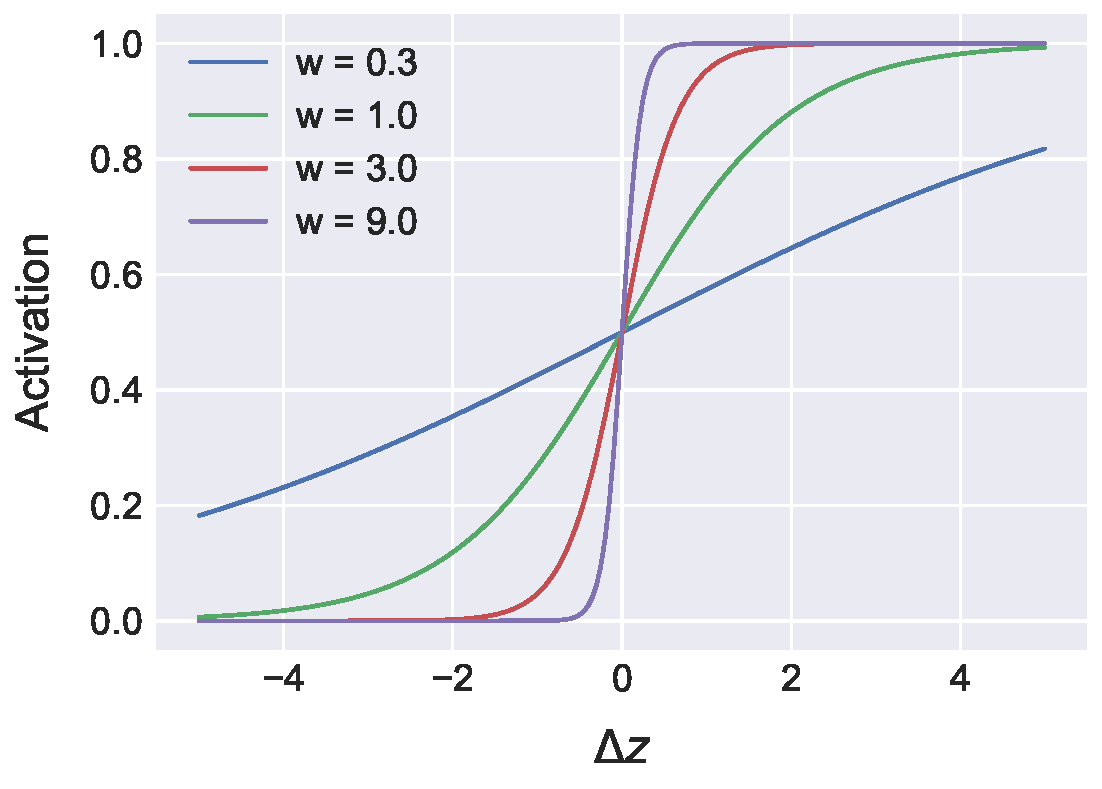
\includegraphics[width=0.5\linewidth]{bin_amp_geo.pdf}
    \caption{\textbf{Geometry of binary softmax cross-entropy after amplification.} Application of different amplification factors $w$ on binary softmax cross-entropy are shown. It can be seen that large $w$'s significantly amplify difference between classes. $w = 1$ means regular softmax cross-entropy.}
    \label{fig:softmax_preamp}
\end{figure}

\paragraph{Adaptive Amplification} Theoretically, an amplification factor $w \to +\infty$ is best suited for the application since the target function approaches classification correctness at the limit. However, the gradient may numerically vanish if $\vdz$ is amplified to a large value. So we need to choose $w$ carefully. Conversely, if the original model outputs a large $\vdz$ which cause the gradient to vanish for a regular cross-entropy, we may be willing to apply a $w < 1$ to let useful gradient information in.

Since differentiation is a linear operator, we may sum up values at different $w$'s. Since we are still willing to approximate the classification correctness as well as we can do, we give larger weights to larger $w$'s. The final loss function is
\begin{equation}
    \mathcal{L}(\vdz) = \sum_{w \in W} w^2 H(\sigma_w(\vdz), y_t),
\end{equation}
where $\vdz$ is the logits before activation, $H$ is cross-entropy function and $y_t$ is ground truth distribution. $W$ is a pre-defined list of possible amplification factors that typically span several orders of magnitude. In the experiments we take $W = [0.3, 1, 2, 3, 4, 5, 6, 7, 8, 9, 10]$.

Note that the forward and backward passes of the entire model only needs to be performed once for the proposed target loss. There is almost no extra computational cost for Adaptive Amplification.

\section*{Appendix: A Krylov Subspace Analysis Method}

The attack based on this analysis is not working well due to the poor approximation of quadratic functions towards neural networks. However, the analysis itself stays interesting, and we thus supply the method in the appendix.

The section is currently pigeoned. Stay tuned.

\end{document}
